\section{Материалы предварительного проектирования системы}
\subsection{Функциональная схема обработки данных}

\begin{figure}[!htb]
    \centering
    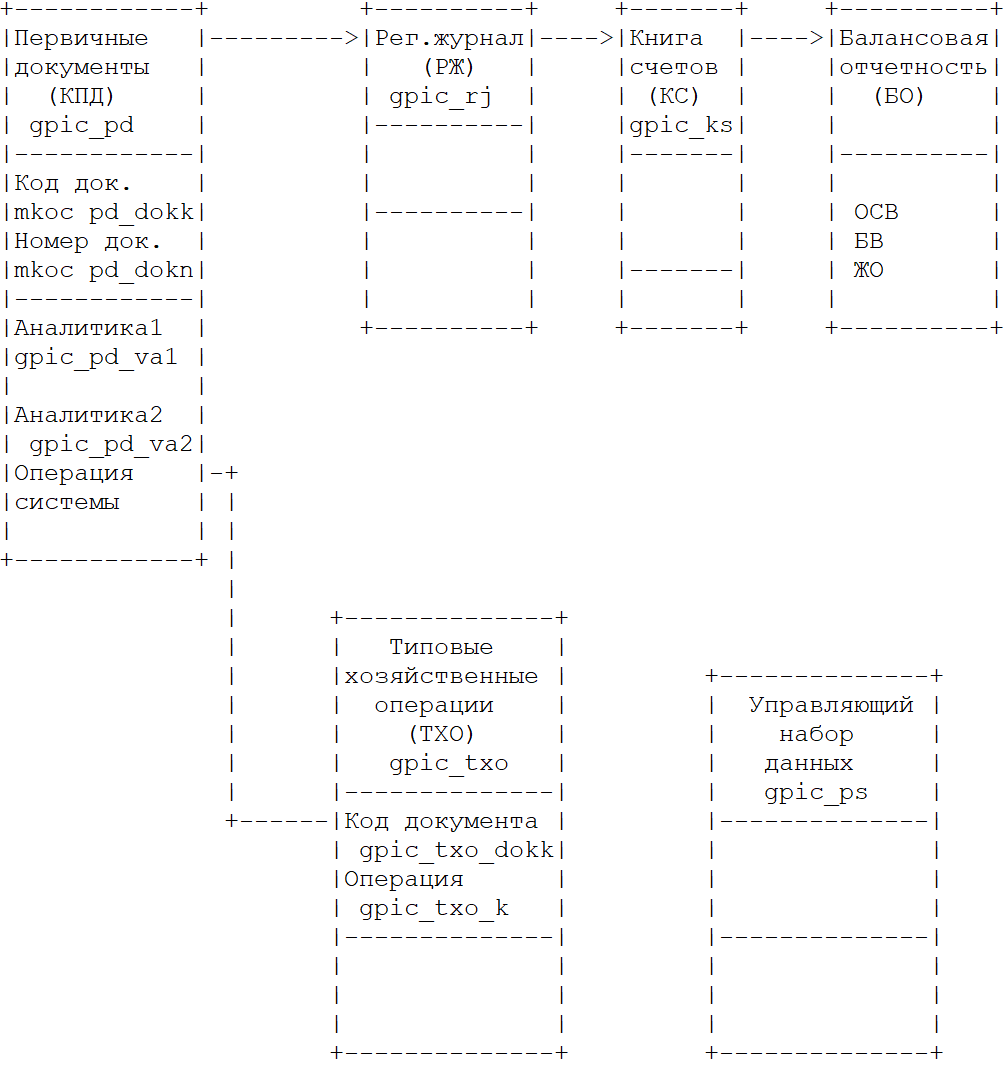
\includegraphics[width=18cm]
        {_assets/gpic_part2.png}
    \caption{Функциональная схема обработки данных}
\end{figure}

\newpage

\subsection{Описание картотек}

Картотеки:

\begin{itemize}
    \item Первичные документы \gpiFIO\/c\_pd;
    \item Регистрационный журнал (РЖ) \gpiFIO\/c\_rj;
    \item Книга счетов (КС) \gpiFIO\/c\_ks;
    \item Типовые хозяйственные операции (ТХО) \gpiFIO\/c\_txo.
\end{itemize}

\begin{table}[h!]
    \centering
    \scriptsize
    \caption{Первичные документы \gpiFIO\/c\_pd}
    \begin{tabular}{|p{7cm}|p{7cm}|c|}

\hline
\multicolumn{1}{|c}{\textbf{Реквизит}}
&\multicolumn{1}{|c}{\textbf{Обозначение}}  
&\multicolumn{1}{|p{1.6cm}|}{\textbf{Тип и значность}} 
\\ \hline

код документа < --- opd             &\gpiFIO\/c\_pd\_dokk   &c7     \\ \hline
номер документа                     &\gpiFIO\/c\_pd\_dokn   &n4     \\ \hline
дата документа                      &\gpiFIO\/c\_pd\_dokd   &n12    \\ \hline
типовая операция < --- txo          &\gpiFIO\/c\_pd\_to     &c10    \\ \hline
дебет *txo                          &\gpiFIO\/c\_pd\_db     &n4     \\ \hline
дебет наименование *txo             &\gpiFIO\/c\_pd\_dbn    &c10    \\ \hline
кредит *txo                         &\gpiFIO\/c\_pd\_kr     &n4     \\ \hline
кредит наименование *txo            &\gpiFIO\/c\_pd\_krn    &c10    \\ \hline
сумма                               &\gpiFIO\/c\_pd\_rub    &n4     \\ \hline

    \end{tabular}
\end{table}

\begin{table}[h!]
    \centering
    \scriptsize
    \caption{Регистрационный журнал (РЖ) \gpiFIO\/c\_rj}
    \begin{tabular}{|p{7cm}|p{7cm}|c|}

\hline
\multicolumn{1}{|c}{\textbf{Реквизит}}
&\multicolumn{1}{|c}{\textbf{Обозначение}}  
&\multicolumn{1}{|p{1.6cm}|}{\textbf{Тип и значность}} 
\\ \hline

дата операции                       &\gpiFIO\/c\_rj\_data   &n12    \\ \hline
код оправдательного документа       &\gpiFIO\/c\_rj\_dokk   &c7     \\ \hline
номер документа                     &\gpiFIO\/c\_rj\_dokn   &n14    \\ \hline
дата документа                      &\gpiFIO\/c\_rj\_dokd   &n12    \\ \hline
содержание операции                 &\gpiFIO\/c\_rj\_to     &c10    \\ \hline
дебет, счет                         &\gpiFIO\/c\_rj\_db     &n4     \\ \hline
дебет, наименование                 &\gpiFIO\/c\_rj\_dbn    &c10    \\ \hline
кредит, счет                        &\gpiFIO\/c\_rj\_kr     &n4     \\ \hline
кредит наименование                 &\gpiFIO\/c\_rj\_krn    &c10    \\ \hline
сумма                               &\gpiFIO\/c\_rj\_rub    &n4     \\ \hline

    \end{tabular}
\end{table}

\begin{table}[h!]
    \centering
    \scriptsize
    \caption{Книга счетов(КС) \gpiFIO\/c\_ks}
    \begin{tabular}{|p{7cm}|p{7cm}|c|}

\hline
\multicolumn{1}{|c}{\textbf{Реквизит}}
&\multicolumn{1}{|c}{\textbf{Обозначение}}  
&\multicolumn{1}{|p{1.6cm}|}{\textbf{Тип и значность}} 
\\ \hline

дата операции                       &\gpiFIO\/c\_ks\_data   &n12    \\ \hline
код оправдательного документа       &\gpiFIO\/c\_ks\_dokk   &c7     \\ \hline
номер документа                     &\gpiFIO\/c\_ks\_dokn   &n4     \\ \hline
дата документа                      &\gpiFIO\/c\_ks\_dokd   &n12    \\ \hline
операции                            &\gpiFIO\/c\_ks\_to     &c10    \\ \hline
счет                                &\gpiFIO\/c\_ks\_s      &n4     \\ \hline
счёт наименование                   &\gpiFIO\/c\_ks\_sn     &c10    \\ \hline
кор. счёт                           &\gpiFIO\/c\_ks\_ks     &n4     \\ \hline
кор. счет наименование              &\gpiFIO\/c\_ks\_ksn    &c10    \\ \hline
сумма дб                            &\gpiFIO\/c\_ks\_rubdb  &n4     \\ \hline
сумма кр                            &\gpiFIO\/c\_ks\_rubkr  &n4     \\ \hline

    \end{tabular}
\end{table}

\begin{table}[h!]
    \centering
    \scriptsize
    \caption{Книга счетов(КС) \gpiFIO\/c\_txo}
    \begin{tabular}{|p{7cm}|p{7cm}|c|}

\hline
\multicolumn{1}{|c}{\textbf{Реквизит}}
&\multicolumn{1}{|c}{\textbf{Обозначение}}  
&\multicolumn{1}{|p{1.6cm}|}{\textbf{Тип и значность}} 
\\ \hline

код документа < --- opd             &\gpiFIO\/c\_txo\_dokk  &c7     \\ \hline
код типовой операции                &\gpiFIO\/c\_txo\_k     &c10    \\ \hline
дебет, счёт < --- ps\_1             &\gpiFIO\/c\_txo\_db    &n4     \\ \hline
дебет, наименование * ps\_1         &\gpiFIO\/c\_txo\_dbn   &c10    \\ \hline
кредит < --- ps\_2                  &\gpiFIO\/c\_txo\_kr    &n4     \\ \hline
кредит, наименование * ps\_2        &\gpiFIO\/c\_txo\_krn   &c10    \\ \hline

    \end{tabular}
\end{table}

\newpage

\subsection{Описание работ}

\begin{table}[h!p]
    \centering
    \scriptsize
    \caption{Описание работ}
    \begin{tabular}{|p{6cm}|p{11cm}|} 

% = = = = = = = = = =

\hline
\multicolumn{1}{|c}{\textbf{Группа работ}}
&\multicolumn{1}{|c|}{\textbf{Работы}}
\\ \hline

% = = = = = = = = = =

Формирование и разноска первичных \par
документов \par
\hspace{0pt} \par
\textbf{\gpiFIO\/c\_Документы}
&
- \gpiFIO\/c\_Ввод текущей даты \par
- \gpiFIO\/c\_Ввод и разноска первичных документов(ПД)
\\ \hline

% = = = = = = = = = =

Работа с регистрационным журналом \par
\hspace{0pt} \par
\textbf{\gpiFIO\/c\_РЖ}
&
- \gpiFIO\/c\_Просмотр РЖ \par
- \gpiFIO\/c\_Формирование КС из РЖ \par
- \gpiFIO\/c\_Просмотр КС
\\ \hline

% = = = = = = = = = =

Формирование балансовой отчетности \par
\hspace{0pt} \par
\textbf{\gpiFIO\/c\_БО}
&
- \gpiFIO\/c\_Опеделение отчетных форм \par
- \gpiFIO\/c\_ОСВ \par
- \gpiFIO\/c\_БВ \par
- \gpiFIO\/c\_Ж-О
\\ \hline

% = = = = = = = = = =

Сопровождение картотек-справочников \par
\hspace{0pt} \par
\textbf{\gpiFIO\/c\_Картотеки}
&
- \gpiFIO\/c\_Типовые хозяйственные операции(ТХО) \par
- \gpiFIO\/c\_Настройка АРМа
\\ \hline

% = = = = = = = = = =

Ведение архивов \par
\hspace{0pt} \par
\textbf{\gpiFIO\/c\_Архивы}
&
- \gpiFIO\/c\_Копия \par
- \gpiFIO\/c\_Восстановление
\\ \hline

% = = = = = = = = = =

Выход из системы \par
\hspace{0pt} \par
\textbf{\gpiFIO\/c\_Выход}
&
- \gpiFIO\/c\_Выход
\\ \hline

% = = = = = = = = = =

    \end{tabular}
\end{table}

\newpage
